%%%%%%%%%%%%%%%%%%%%%%%%%%%%%%%%%%%%%%%%%%%%%%%%%%%%%%%%%%%%%%%%%%%%%%%%%%%%%% 
%%%%%%%%%%%%%%%%%%%%%%%%%%%%%%%%%%%%%%%%%%%%%%%%%%%%%%%%%%%%%%%%%%%%%%%%%%%%%%



%%%%%%%%%%%%%%%%%%%%%%%%%%%%%%%%%%%%%%%%%%%%%%%%%%%%%%%%%%%%%%%%%%%%%%%%%%%%%%
%               Globale Einstellungen für das Dokument
%%%%%%%%%%%%%%%%%%%%%%%%%%%%%%%%%%%%%%%%%%%%%%%%%%%%%%%%%%%%%%%%%%%%%%%%%%%%%%

\documentclass[12pt,a4paper]{article}
%\usepackage[utf8]{inputenc}
\usepackage[T1]{fontenc}        % Zeichenenkodierung definieren
\usepackage[ngerman]{babel}     % neue Rechtschreibung verwenden
\usepackage{amsmath}            % zusätzliche mathematische Symbole
\usepackage{amsthm}
\usepackage{amsfonts}
\usepackage{amsrefs}
\usepackage{amssymb}
%\usepackage{uniinput}
\usepackage[table]{xcolor}
\usepackage{graphicx}           % Grafiken ermöglichen
\usepackage{fancyvrb}           % Verbose-Modus verschönern
\usepackage{fancyhdr}
\usepackage{listings}
\usepackage{xunicode}
\usepackage{xltxtra}
\usepackage{fontspec}
\usepackage{libertine}
\usepackage{hyperref}
\usepackage[toc]{glossaries}
\usepackage[compact]{titlesec}
\usepackage{titletoc}
\usepackage{hhline}
\usepackage{ifthen}

\usepackage[top=45mm, left=40mm, right=40mm, bottom=45mm,
headheight=1cm, headsep=1cm, footskip=1.2cm]{geometry}

\newboolean{blackwhite}
\setboolean{blackwhite}{false}

%%%%%%%%%%%%%%%%%%%%%%%%%%%%%%%%%%%%%%%%%%%%%%%%%%%%%%%%%%%%%%%%%%%%%%%%%%%%
% Farbdefinitionen

\ifthenelse{\boolean{blackwhite}}
{
% define colors for listings
\definecolor{black}{rgb}{0,0,0}
\definecolor{colKeys}{rgb}{0,0,0}
\definecolor{colIdentifier}{rgb}{0,0,0}
\definecolor{colComments}{rgb}{0,0,0}
\definecolor{colString}{rgb}{0,0,0}

% define colors for text usage
\definecolor{section}{rgb}{0,0,0}
\definecolor{colTitle}{rgb}{0,0,0}
\definecolor{colHeadrule}{rgb}{0, 0, 0}
\definecolor{colFootrule}{rgb}{0, 0, 0}
\Definecolor{colPart}{rgb}{0,0,0}
\definecolor{colPartRule}{rgb}{0, 0, 0}
\definecolor{colSection}{rgb}{0,0,0}
\definecolor{colSectionRule}{rgb}{0, 0, 0}
\definecolor{colSubsection}{rgb}{0,0,0}
\definecolor{colSubsubsection}{rgb}{0, 0, 0}
\definecolor{colDefinition}{rgb}{0,0,0}
\definecolor{colTableHeader}{rgb}{0, 0, 0}
\definecolor{colRow}{rgb}{0,0,0}
\definecolor{colColumn}{rgb}{0,0,0}
\definecolor{colTableBright}{rgb}{0.8, 0.8, 0.8}
\definecolor{colTableDark}{rgb}{0.0, 0.0, 0.0}
\definecolor{colTableRule}{rgb}{0.0, 0.0, 0.0}
\definecolor{colListingBackground}{rgb}{0, 0, 0}
\definecolor{colListingRule}{rgb}{0, 0, 0}
\definecolor{colPageNumber}{rgb}{0,0,0}
\definecolor{colHeadNote}{rgb}{0, 0, 0}
\definecolor{colHrule}{rgb}{0,0,0}
}
{

% Define colors for listings
\definecolor{black}{cmyk}{0.0, 0.0, 0.0, 1.0}
\definecolor{colKeys}{rgb}{0,0,1}
\definecolor{colIdentifier}{rgb}{0,0,0}
\definecolor{colComments}{rgb}{0,0.5,0}
\definecolor{colString}{rgb}{0.7,0,0}

% define colors for text usage
\definecolor{section}{cmyk}{1.0, 0.33, 0, 0.25}
\definecolor{colTitle}{rgb}{0,0.31373,0.37451}
\definecolor{colHeadrule}{cmyk}{1.0, 0.33, 0, 0.25}
\definecolor{colFootrule}{cmyk}{1.0, 0.33, 0, 0.25}
\definecolor{colPart}{rgb}{0,0.31373,0.47451}
\definecolor{colPartRule}{cmyk}{1.0, 0.33, 0, 0.25}
\definecolor{colSection}{rgb}{0,0.31373,0.47451}
\definecolor{colSectionRule}{cmyk}{1.0, 0.33, 0, 0.25}
\definecolor{colSubsection}{rgb}{0,0.40784,0.61569}
\definecolor{colSubsubsection}{cmyk}{1.0, 0.33, 0, 0.25}
\definecolor{colDefinition}{rgb}{0,0.31373,0.47451}
\definecolor{colTableHeader}{cmyk}{0.19608, 0.0078431, 0.0, 0.0}
\definecolor{colRow}{rgb}{0.77255, 0.92549, 1.0}
\definecolor{colColumn}{rgb}{0.77255, 0.92549, 1.0}
\definecolor{colTableBright}{cmyk}{0.19608, 0.0078431, 0.0, 0.0}
\definecolor{colTableDark}{cmyk}{1.0, 0.33, 0, 0.25}
\definecolor{colTableRule}{cmyk}{1.0, 0.33, 0, 0.25}
\definecolor{colListingBackground}{cmyk}{0.19608, 0.0078431, 0.0, 0.0}
\definecolor{colListingRule}{cmyk}{1.0, 0.33, 0, 0.25}
\definecolor{colPageNumber}{rgb}{0,0.40784,0.61569}
\definecolor{colHeadNote}{cmyk}{1.0, 0.33, 0, 0.25}
\definecolor{colHrule}{rgb}{0,0.40784,0.61569}
}

%%%%%%%%%%%%%%%%%%%%%%%%%%%%%%%%%%%%%%%%%%%%%%%%%%%%%%%%%%%%%%%%%%%%%%%%%%%%
% Tabellen

\renewcommand{\arrayrulewidth}{1pt}

\arrayrulecolor{colTableRule}

% \newcommand\tableline{%
%   \hhline{
%     >{\arrayrulecolor{colTableRule}\doublerulesepcolor{colTableRule}}%
%     -%
%     >{\arrayrulecolor{colTableRule}\doublerulesepcolor{colTableRule}}%
%     -%
%   }}



%%%%%%%%%%%%%%%%%%%%%%%%%%%%%%%%%%%%%%%%%%%%%%%%%%%%%%%%%%%%%%%%%%%%%%%%%%%%

\lstset{%
    float=hbp,%
    basicstyle=\color{black}\small, %
    identifierstyle=\color{colIdentifier}, %
    keywordstyle=\color{colKeys}, %
    stringstyle=\itshape\color{colString}, %
    commentstyle=\color{colComments}, %
    columns=fullflexible, %
    tabsize=1, %
    frame=single, %
    extendedchars=true, %
    showspaces=false, %
    showstringspaces=false, %
    numbers=left, %
    numberstyle=\tiny, %
% backgroundcolor=\color{colListingBackground},
    breaklines=true, %
    breakautoindent=true, %
    captionpos=b,%
    rulecolor=\color{colListingRule},%
    frameround=tttt
}


% PDFAuthor einfügen

\usepackage{float}
%\usepackage{picins}             % Textumfluss ermöglichen
                                % Ränder einstellen


\parindent0cm                   % Erstzeileneinzug ausschalten
\fvset{fontsize=\scriptsize,frame=single,numbers=left}

\numberwithin{equation}{section}
\numberwithin{table}{subsection}
%%%%%%%%%%%%%%%%%%%%%%%%%%%%%%%%%%%%%%%%%%%%%%%%%%%%%%%%%%%%%%%%%%%%%%%%%%%%%%
%                            Makros definieren
%%%%%%%%%%%%%%%%%%%%%%%%%%%%%%%%%%%%%%%%%%%%%%%%%%%%%%%%%%%%%%%%%%%%%%%%%%%%%%

\newenvironment{definition}[1]{
  \textbf{Definition #1}    
}{
\bigskip

}

\newenvironment{bemerkung}{
  \textbf{Bemerkung}    
}{
\bigskip

}

%\setmainfont[Mapping=tex-text]{Linux Libertine}
%\newfontface\fancy[Contextuals={WordInitial,WordFinal}]{AJensonPro-SemiboldIt} 
\newcommand*{\tableheader}[1]{\color{colTableDark}\textsf{\textit{\textbf{#1}}}}
\newcommand*{\colhrule}{\vbox to 1pt{\hbox
    to\textwidth{\textcolor{colHrule}{\hrulefill}}\vss}}

%%%%%%%%%%%%%%%%%%%%%%%%%%%%%%%%%%%%%%%%%%%%%%%%%%%%%%%%%%%%%%%%%%%%%%%%%%%%
% Aussehen der Überschriften definieren

%\titleformat{\part}[block]{\Large \it \bfseries}{\thepart}{.5em}{}

%\titlecontents{\part}[display]{\textcolor{blue}}{}{}{\titlerule}
\titlecontents{part}
[0em]
{\vspace{0.7cm}\color{colPart}\large\sffamily}
{\contentslabel{2.3em}}
{\hspace*{-1.3em}}%
{\normalfont\hfill\color{black}\contentspage}%\titlerule*[0.11pc]{.}

\titlecontents{section}
[0em]
{\vspace{0.5cm}\color{colSection}\sffamily}
{\contentslabel{1.6em}}
{\hspace*{-0.0em}}%
{\normalfont\hfill\bfseries\color{black}\contentspage}%\titlerule*[0.11pc]{.}

\titlecontents{subsection}
[3.0em]
{\color{black}\sffamily}
{\contentslabel{2.0em}}
{\hspace*{4.5em}}%
{\normalfont\color{colSubsection}\dotfill\color{black}\contentspage}

\titlecontents{subsubsection}
[6.0em]
{\color{black}\sffamily}
{\contentslabel{3em}}
{\hspace*{5.0em}}%
{\normalfont\color{colSubsection}\dotfill\color{black}\contentspage}


\titleformat{\part}[display]
{\color{colPart}\normalfont\Large\filcenter\sffamily}
{\color{colPartRule}\titlerule[1pt]%
\vspace{1pt}%
\titlerule
\vspace{1pc}%
\color{colPart}\LARGE\MakeUppercase{\partname} \thepart
}
{0pc
}
{\color{colPartRule}\titlerule
\vspace{1pc}%
\color{colPart}\Huge}

\titleformat{\subsection}[display]
{\bf\sffamily}
{}
{0mm}
{\large \color{colSubsection}\thesubsection~~
}

\titleformat{\subsubsection}[display]
{\bf\sffamily}
{}
{0pc}
{\color{colSubsubsection}\thesubsubsection~~
}

% \renewcommand{\thepart}{\Roman{part}}
% \titleformat{\part}[display]
% {\bfseries\Large}
% {\filleft\MakeUppercase{\partname} \Huge \thepart}
% {4ex}
% {\titlerule
%   \vspace{2ex}%
%   \filright}
% [\vspace{2ex}%
% \titlerule]


%%%%%%%%%%%%%%%%%%%%%%%%%%%%%%%%%%%%%%%%%%%%%%%%%%%%%%%%%%%%%%%%%%%%%%%%%%%%

\newtheoremstyle{mdef}{3ex} {3ex} {\slshape}{} %
% UeFont     Trenn   AbstUe     UeBefs
    {}        {:}   {\newline}    {}
\theoremstyle{mdef}
\newtheorem{mthm}{\color{colDefinition}\textbf{Definition}}[section]
\newtheorem{msatz}{\textbf{Satz}}
\newtheorem{mbeweis}{\textbf{Beweis}}
\newtheorem{mrmk}{\textbf{Bemerkung}}

\newglossary[slg]{symbols}{sym}{sbl}{List of Symbols}

%%%%%%%%%%%%%%%%%%%%%%%%%%%%%%%%%%%%%%%%%%%%%%%%%%%%%%%%%%%%%%%%%%%%%%%%%%%%%%

\begin{document}

%%%%%%%%%%%%%%%%%%%%%%%%%%%%%%%%%%%%%%%%%%%%%%%%%%%%%%%%%%%%%%%%%%%%%%%%%%%%%%
%                          Titelseite generieren
%%%%%%%%%%%%%%%%%%%%%%%%%%%%%%%%%%%%%%%%%%%%%%%%%%%%%%%%%%%%%%%%%%%%%%%%%%%%%%

\vspace{-1cm}
\enlargethispage{3cm}
\begin{titlepage}
    \colhrule
    \begin{center}    
      {\color{colTitle}\Large \bf\sffamily 
        RGBLightControl}
      \colhrule
      \vspace*{1.7cm}
      {\Large \textsc{Manual}\vspace{0.2cm}}\\
      \vspace{0.2cm}
      
      \vspace*{0.4cm}

      \vspace*{0.4cm}
      
      \vspace{0.4cm}
      
      \begin{figure}[H]
        \centering
        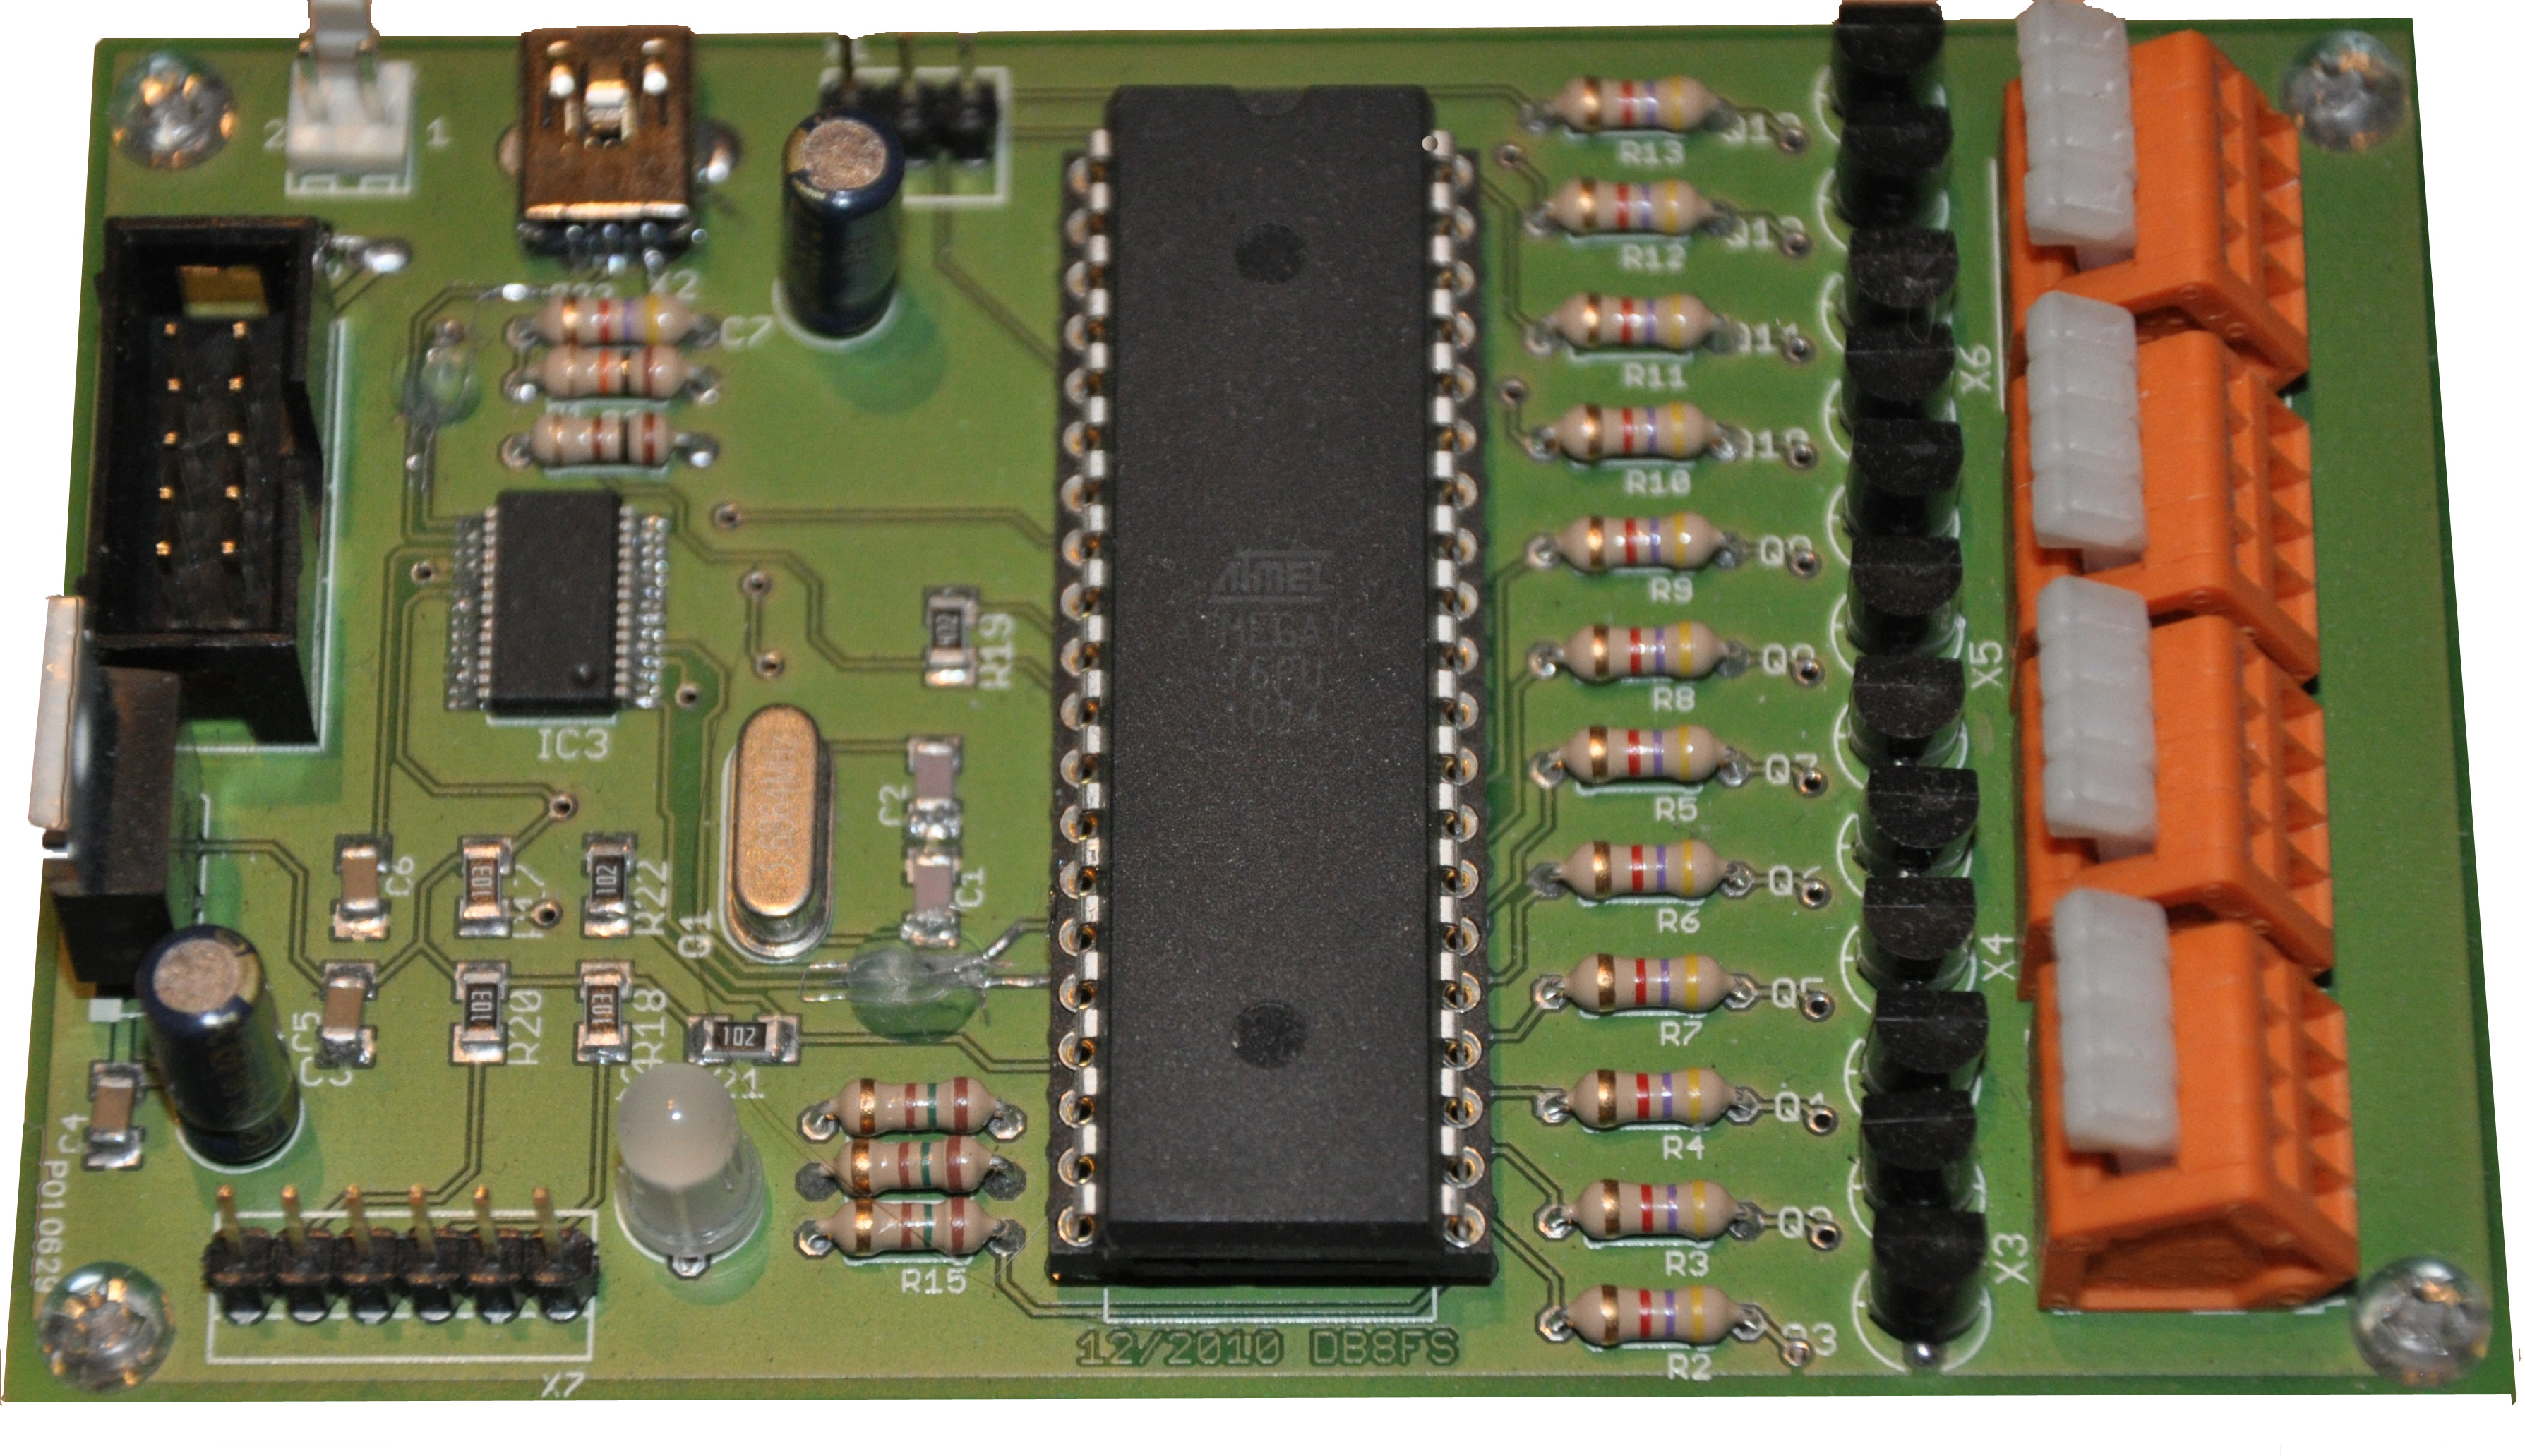
\includegraphics[scale=0.3]{images/Platine-Screenshot.jpg}
      \end{figure}
      
      \vspace{0.4cm}
      
      \textbf{\textsf{\small Version 0.1}}
      \vspace{1.0cm}

      \textbf{\textsf{\small Falk Schilling (DB8FS)}}
      \vspace{1.0cm}

      \textbf{\textsf{\small \today}}
      \vspace{0.4cm}
      

      \vspace{2.2cm} 
    \end{center}
    \colhrule
\end{titlepage}


%%%%%%%%%%%%%%%%%%%%%%%%%%%%%%%%%%%%%%%%%%%%%%%%%%%%%%%%%%%%%%%%%%%%%%%%%%%%%
% Stil für Sektionsseiten anpassen
%%%%%%%%%%%%%%%%%%%%%%%%%%%%%%%%%%%%%%%%%%%%%%%%%%%%%%%%%%%%%%%%%%%%%%%%%%%%%

\fancypagestyle{plain}{%
\fancyhf{} % clear all header and footer fields
%\fancyfoot[R]{\slshape \textcolor{colPageNumber} \thepage}
\renewcommand{\headrule}{}
\renewcommand{\headrulewidth}{0pt}
\renewcommand{\footrulewidth}{0.2pt}}

%%%%%%%%%%%%%%%%%%%%%%%%%%%%%%%%%%%%%%%%%%%%%%%%%%%%%%%%%%%%%%%%%%%%%%%%%%%%%%
%              Kopf- und Fußzeilen, Seitenzahlen anpassen
%%%%%%%%%%%%%%%%%%%%%%%%%%%%%%%%%%%%%%%%%%%%%%%%%%%%%%%%%%%%%%%%%%%%%%%%%%%%%%

\pagestyle{fancy}
% % Markierungen setzen für Fuß- und Kopfzeilen
\renewcommand{\partmark}[1]{}
\renewcommand{\subsectionmark}[1]{\markright{#1}}

% % Inhalte der Kopf- und Fußzeilen festlegen
\lhead[]{} 
\chead{}
\rhead[]{\color{colHeadNote}\textsl{\nouppercase{\leftmark}}}

\lfoot[]{}
 \cfoot[]{}
 \rfoot[]{\slshape \textcolor{colPageNumber} \thepage}

\renewcommand{\headrule}{\vbox to 0pt{\hbox
to\headwidth{\textcolor{colHeadrule}{\hrulefill}}\vss}}

\renewcommand{\footrule}{\vbox to 0pt{\hbox
to\headwidth{\textcolor{colFootrule}{\hrulefill}}\vss}} 

\renewcommand{\headrulewidth}{0.2pt}
\renewcommand{\footrulewidth}{0.2pt}


%%%%%%%%%%%%%%%%%%%%%%%%%%%%%%%%%%%%%%%%%%%%%%%%%%%%%%%%%%%%%%%%%%%%%%%%%%%%%
\titleformat{\section}[display] % command shape
{\bf\sffamily} % format
{} % label
{0pc} % seperator
{\hfill\Large \color{colSection}}
[{\color{colSectionRule}\titlerule[1pt]\vspace{0.6cm}}]
%\titlerule[0.2pt]\vspace{1pt}}

\section*{Zusammenfassung}
\thispagestyle{plain}
Dieses Dokument beschäftigt sich mit dem Hardwareaufbau und der Firmware
eines Atmel ATmega16 basierenden Steuerungsmoduls für RGB-LEDs mit
maximal 4 Kanälen. Desweiteren soll eine mögliche Anwendung in
Kombination mit dem Festplattenreceiver DM8000 der Dream Multimedia
GmbH gezeigt werden.

\titleformat{\section}[display] % command shape
{\bf\sffamily} % format
{} % label
{0pc} % seperator
{\Large \color{colSection}}
[{\color{colSectionRule}\titlerule[1pt]\vspace{0.6cm}}]
%\titlerule[0.2pt]\vspace{1pt}}



\clearpage
\thispagestyle{plain}
\tableofcontents
\clearpage

%%%%%%%%%%%%%%%%%%%%%%%%%%%%%%%%%%%%%%%%%%%%%%%%%%%%%%%%%%%%%%%%%%%%%%%%%%%%%%
%              Hier den eigentlichen Inhalt einfügen...
%%%%%%%%%%%%%%%%%%%%%%%%%%%%%%%%%%%%%%%%%%%%%%%%%%%%%%%%%%%%%%%%%%%%%%%%%%%%%%
\section{Grundlagen}

\subsection{Pulsweitenmodulation}

\clearpage


\section{Hardware}

\subsection{Anforderungen}

\subsection{Schaltungsentwurf}
%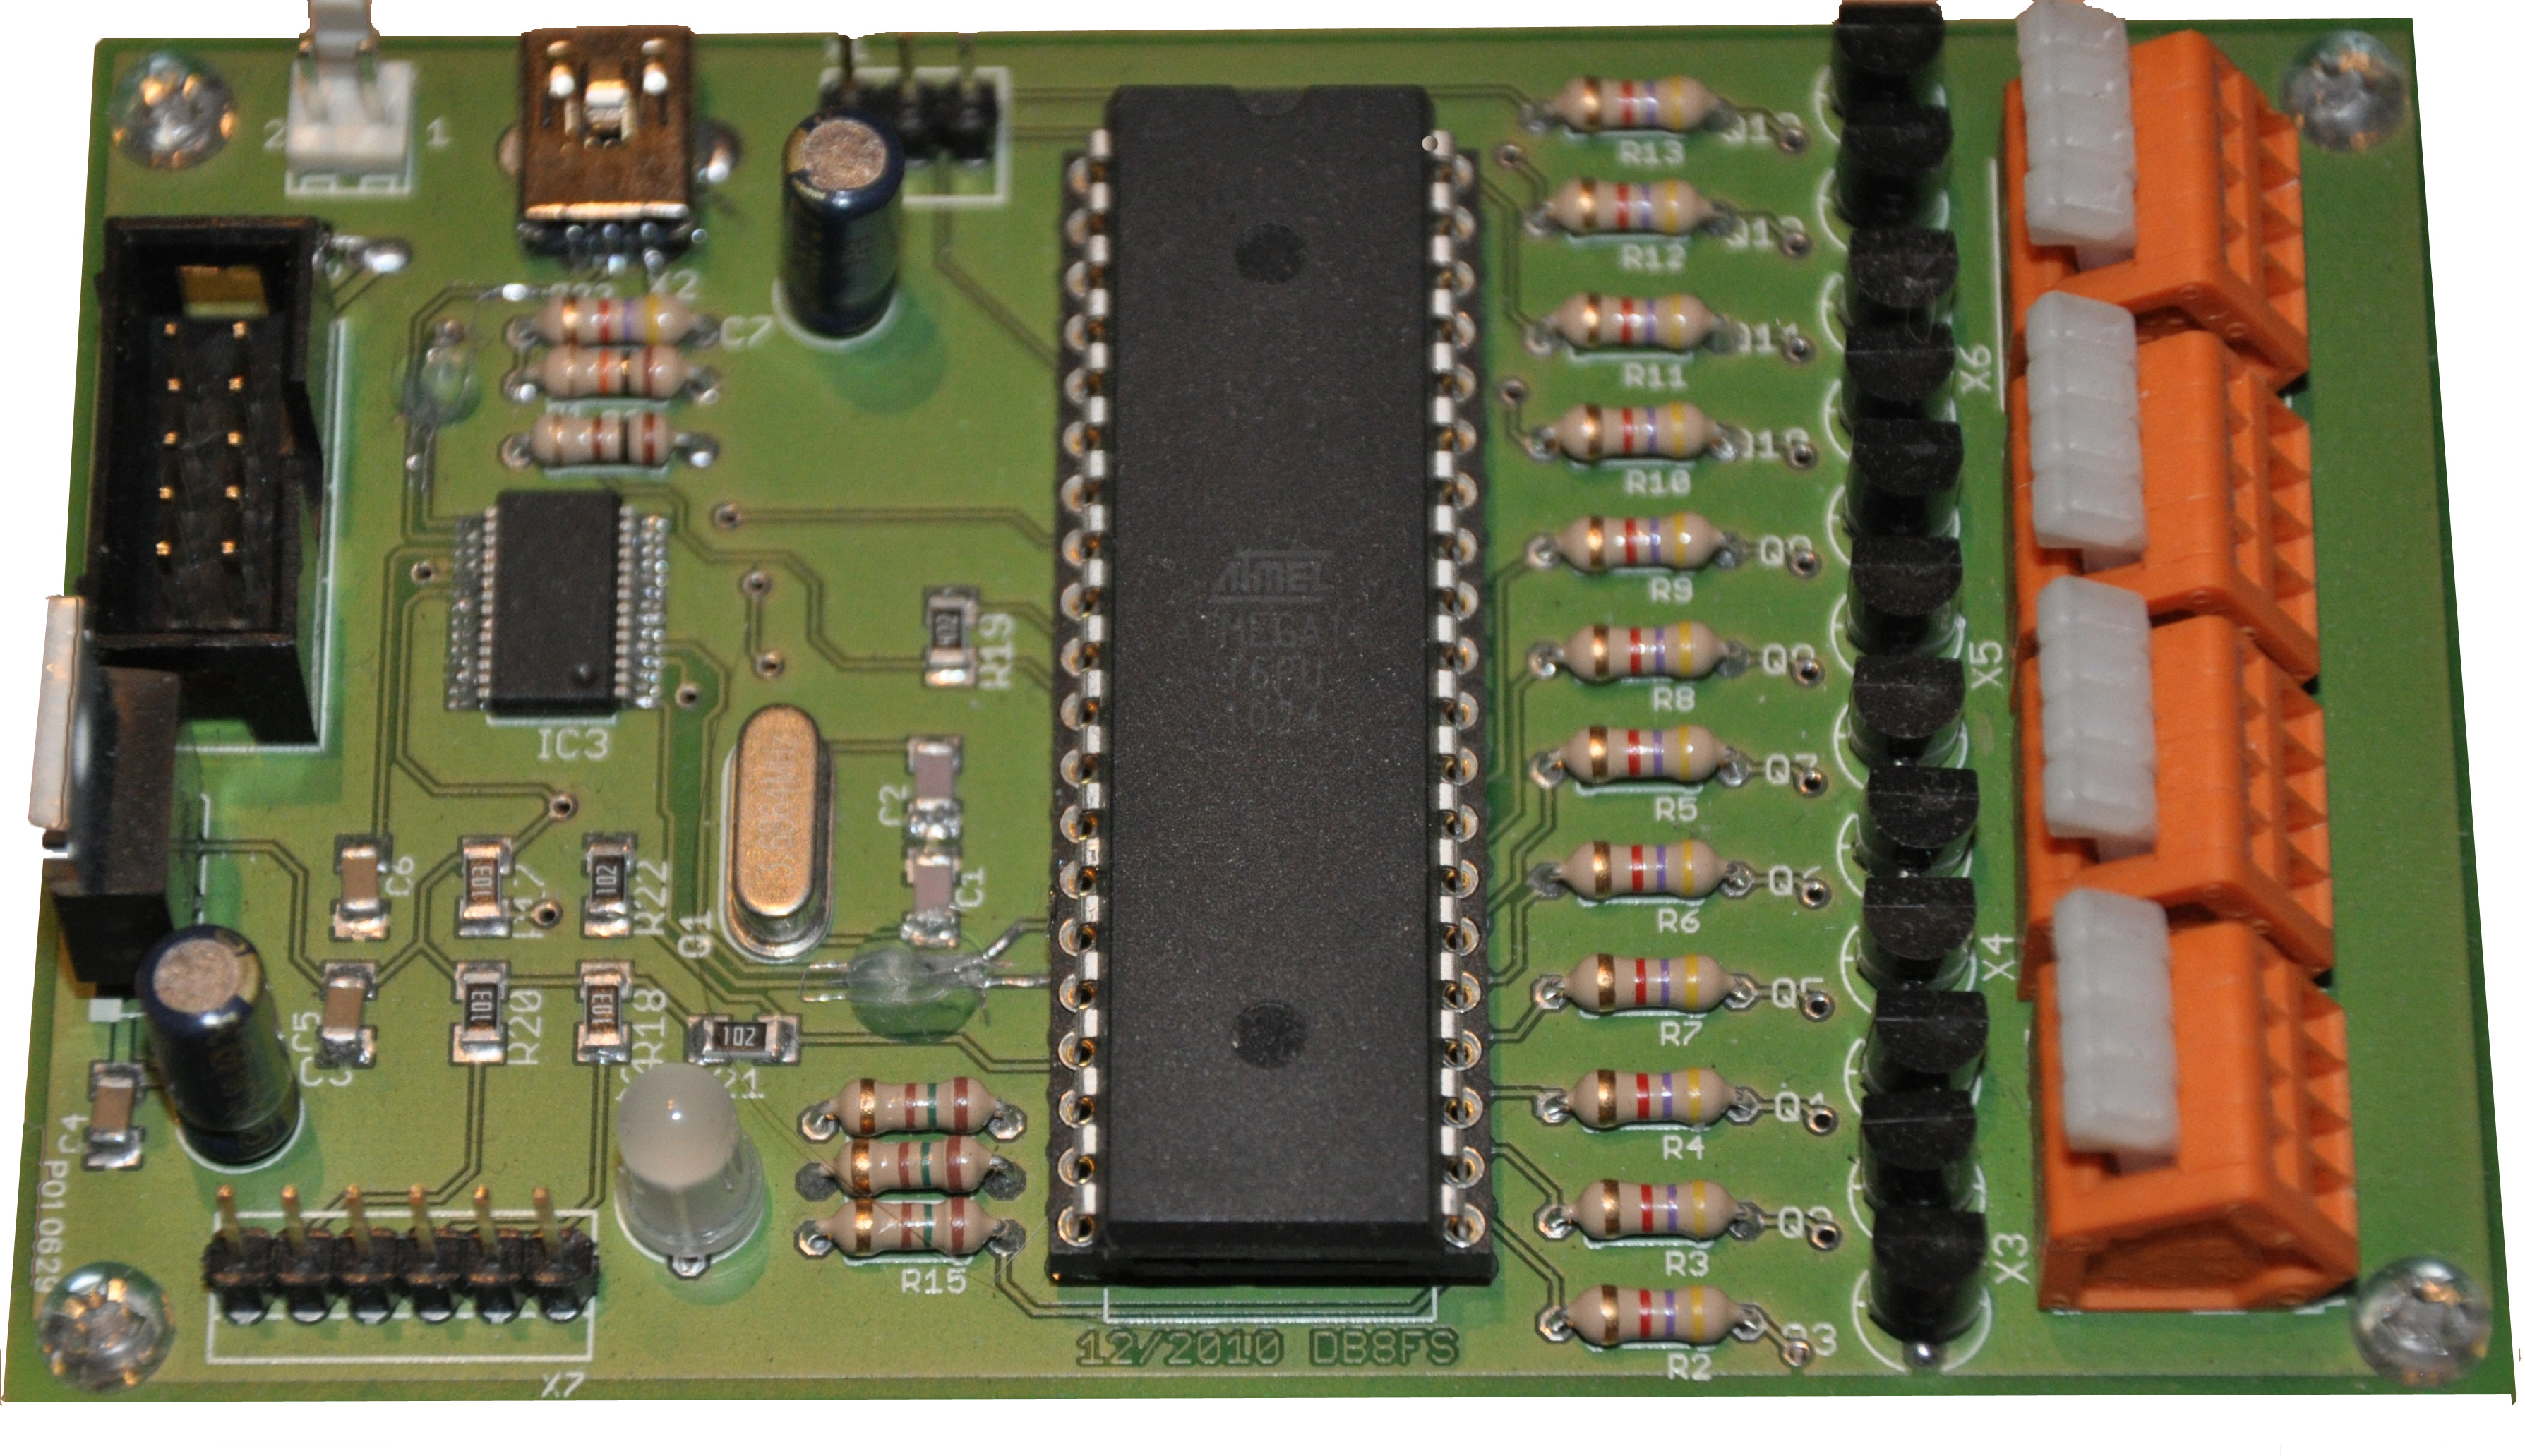
\includegraphics[scale=0.3]{images/Platine-Screenshot.jpg}

\clearpage
\thispagestyle{plain}
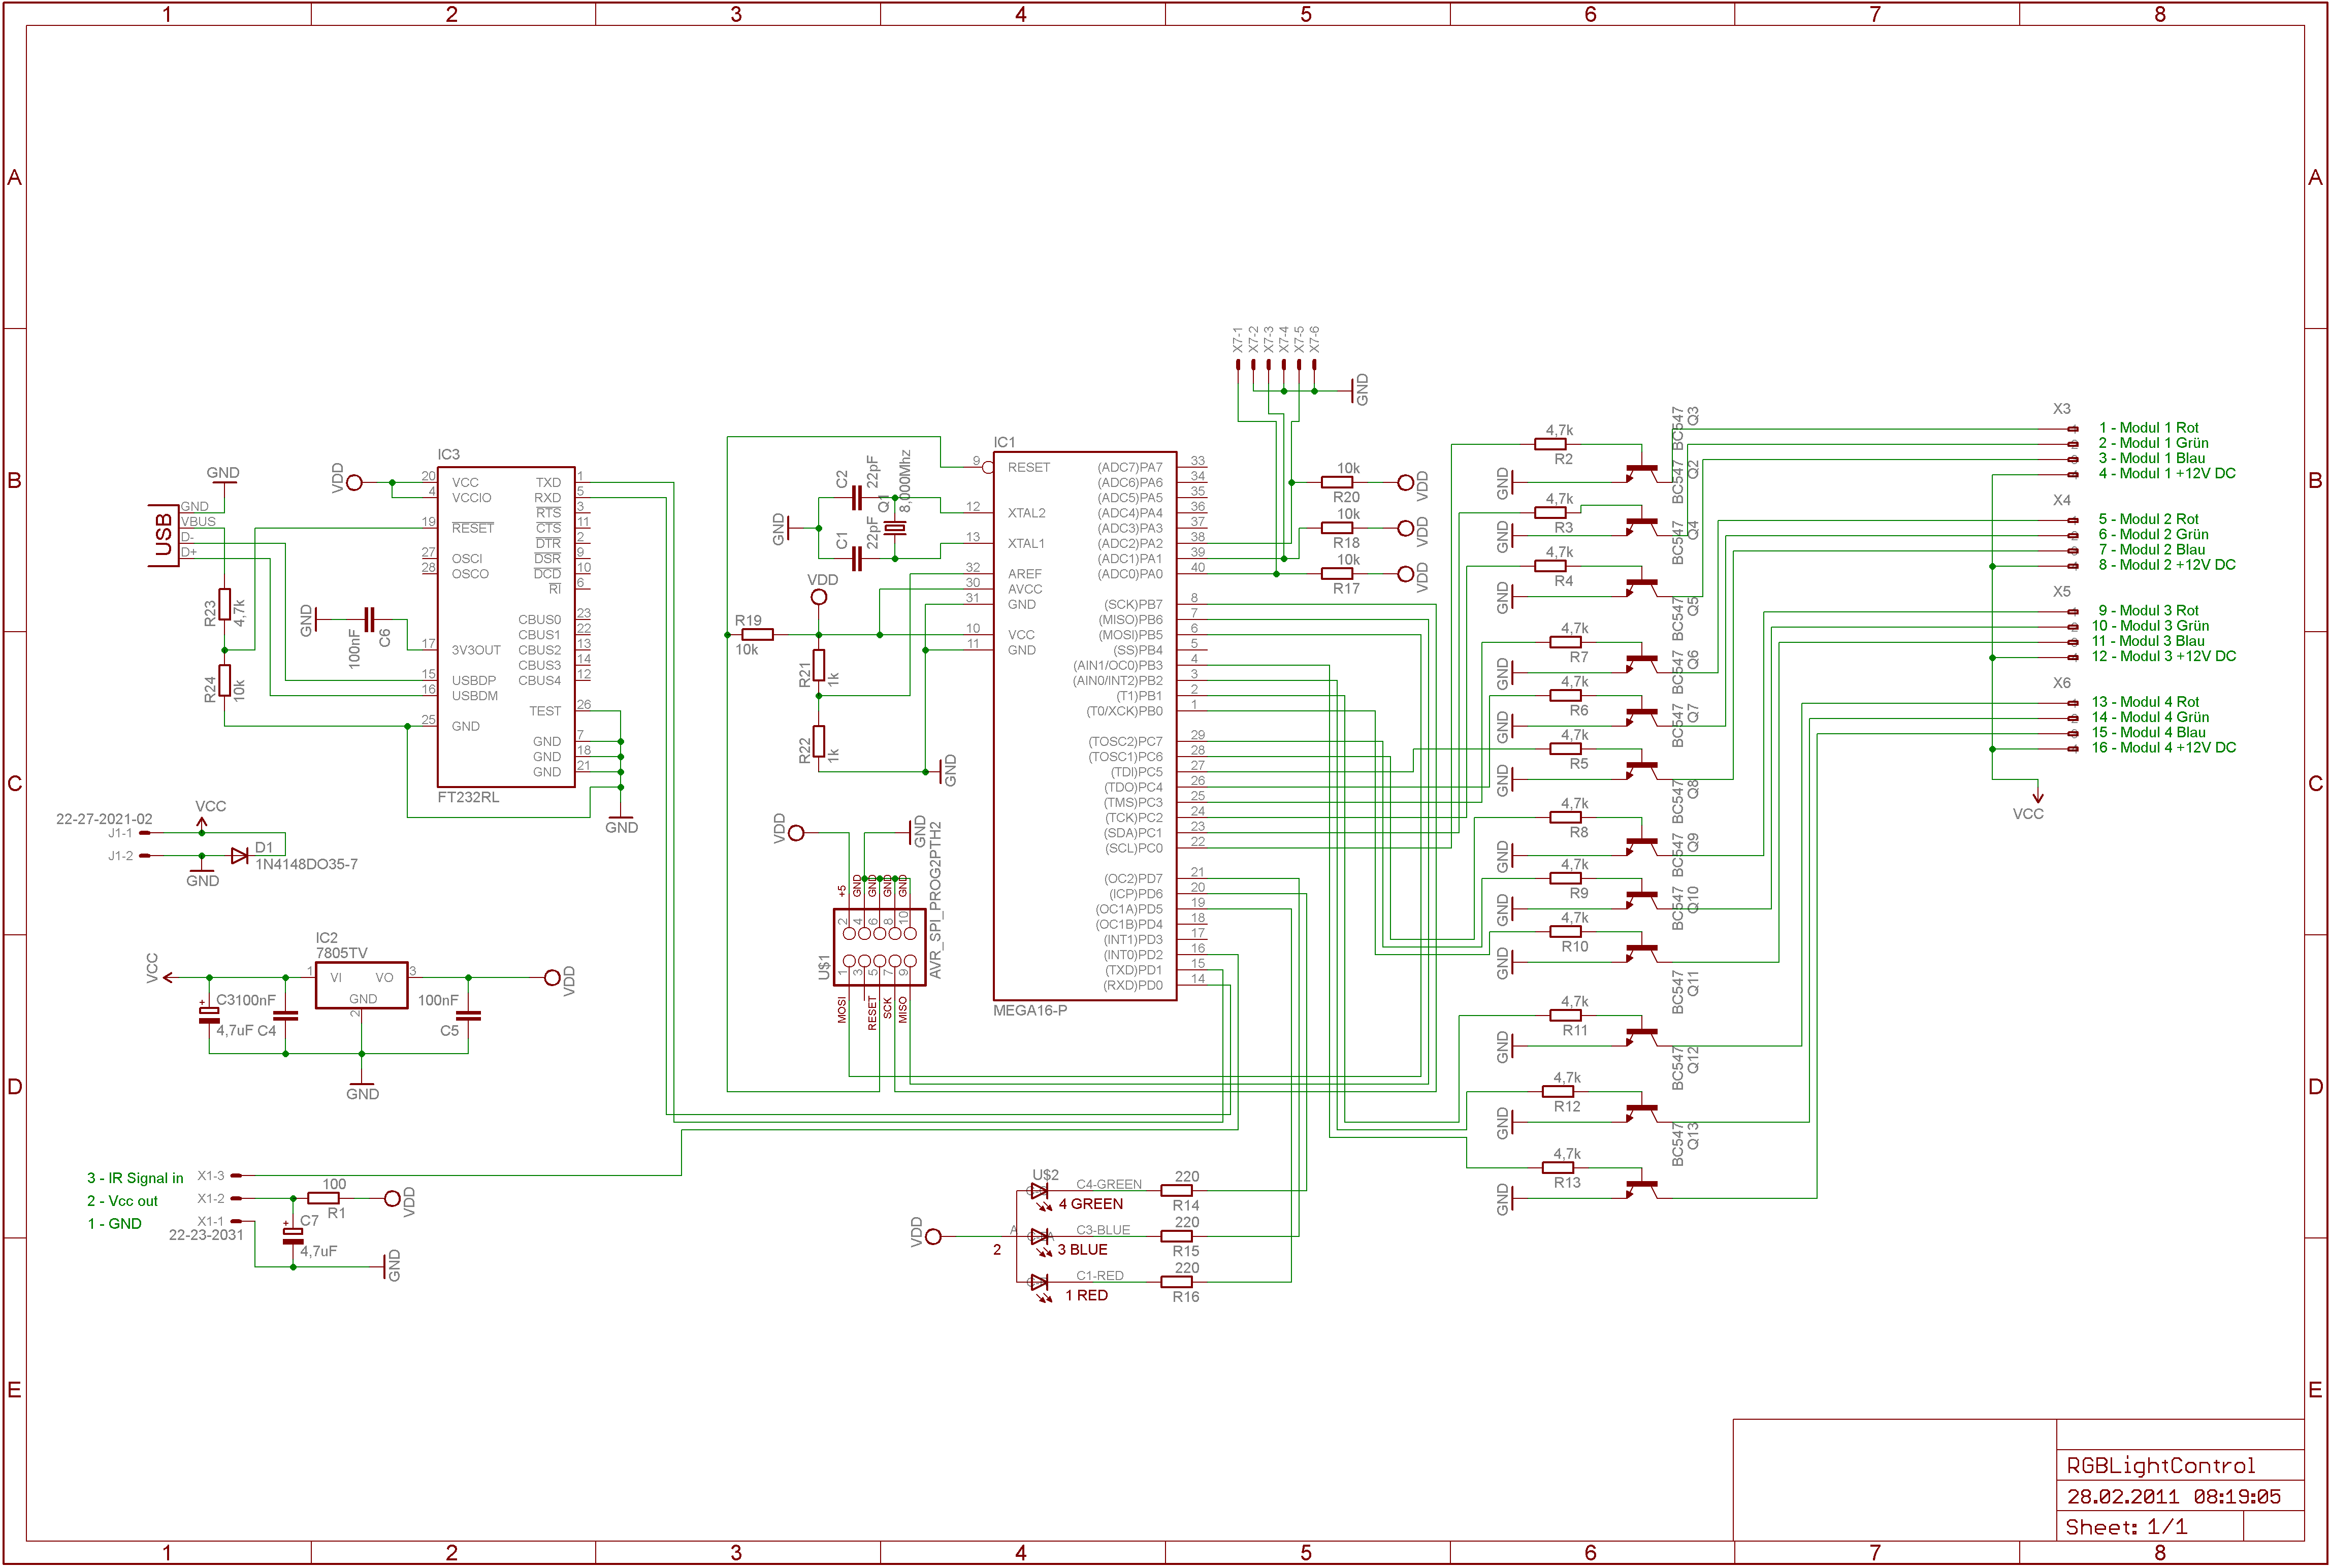
\includegraphics[scale=0.5,angle=90]{images/schematic-large.png}
\clearpage

\subsection{Board-Layout}
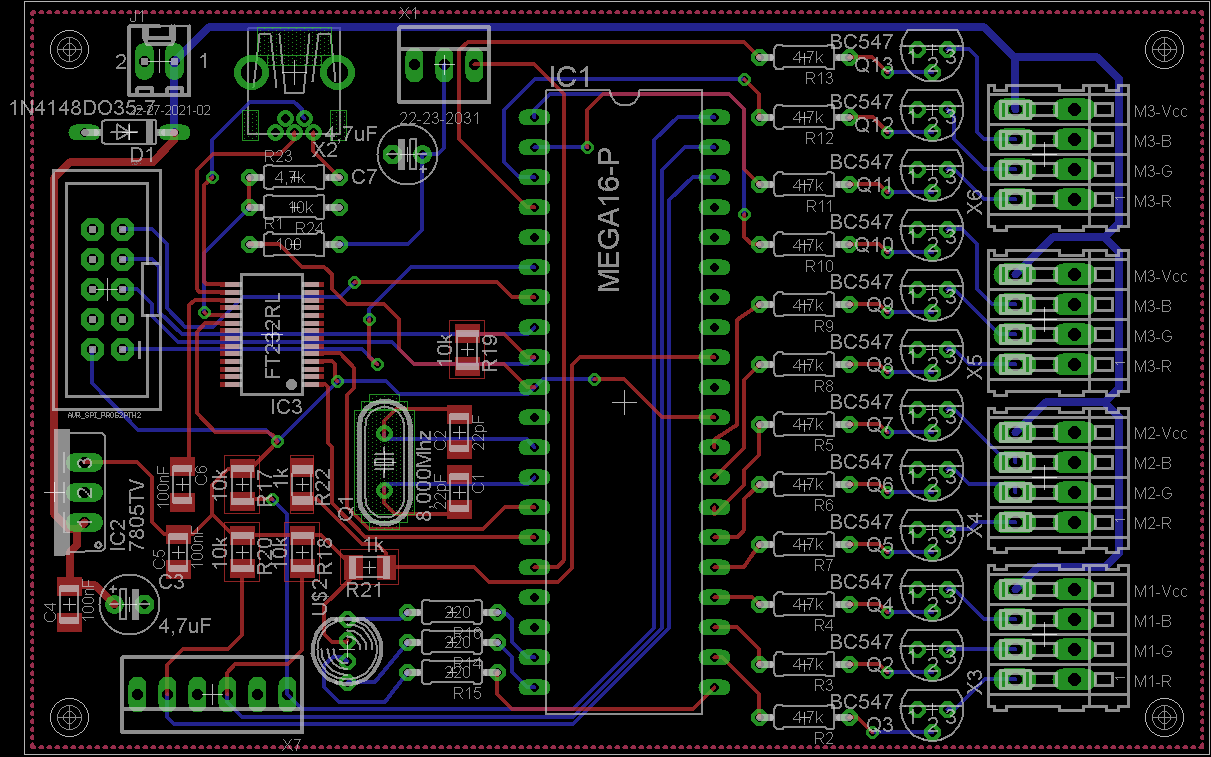
\includegraphics{images/board-large.png}
\clearpage


\section{Firmware}
\clearpage


\section{Software}
\clearpage

%%%%%%%%%%%%%%%%%%%%%%%%%%%%%%%%%%%%%%%%%%%%%%%%%%%%%%%%%%%%%%%%%%%%%%%%%%%%%%
%                         Ende des Dokuments
%%%%%%%%%%%%%%%%%%%%%%%%%%%%%%%%%%%%%%%%%%%%%%%%%%%%%%%%%%%%%%%%%%%%%%%%%%%%%%

\end{document}
